% ------ headers globales -------------
\documentclass[11pt, a4paper, twoside]{article}
\usepackage{header}
\usepackage{config}
% -------------------------------------
\begin{document}

% -- Carátula --
\clearpage{\pagestyle{empty}% parametros para la caratula (caratula.sty)

\materia{Sistemas Operativos}
%\submateria{}
\titulo{Trabajo Práctico 3}
\subtitulo{Algoritmos en sistemas distribuidos}
%\subtitulo{Escape en Sistemas}
\fecha{13 de noviembre de 2014}
\integrante{Rodriguez, Pedro}{197/12}{pedro3110.jim@gmail.com}
\integrante{Benegas, Gonzalo Segundo}{958/12}{gsbenegas@gmail.com}
\integrante{Barrios, Leandro Ezequiel}{404/11}{ezequiel.barrios@gmail.com}
%\grupo{Grupo ??}

\maketitle
\cleardoublepage}

%-- Índice --
\clearpage{%
  \pagestyle{empty}\tableofcontents%
  \vspace{3cm}%
  \begin{abstract}
  En el presente trabajo práctico estudiaremos algunos de los métodos más comúnmente utilizados 
  en la actualidad por distintos sistemas operativos para manejar correcta y eficientemente los 
  diversos procesos que se ejecutan concurrentemente en máquinas con uno o más procesadores.

  Intentaremos detectar las ventajas y desventajas de cada método, así como los escenarios en los
  cuales uno puede ser más eficiente que otro. Para esto, dividimos el TP en tres partes: en la
  primera, presentamos el simulador \texttt{simusched} y lo corremos para algunas tareas específicas. En la
  segunda parte, extendemos el simulador con nuevos schedulers implementados por nosotros y finalmente,
  en la tercera parte evaluamos y analizamos los distintos algoritmos de scheduling ya presentados.
  \end{abstract}
  \cleardoublepage%
}
%-- A partir de aquí, pongo el contador de páginas en 1 --
\setcounter{page}{1}

\index{Entendiendo el simulador simusched}
\section{Entendiendo el simulador simusched}

\subsection{Ejercicio 1}
En este ejercicio, programamos la tarea \texttt{TaskConsola}, que simularía una tarea interactiva con
el usuario. 

Para la implementación de esta tarea, primero tuvimos que registrarla para que el simulador la 
reconozca en el archivo \texttt{tasks.cpp}, con la función \texttt{tasksinit(void)}. En ese mismo archivo implementamos
la tarea, que para el proceso número $pid$ recibe los tres parámetros: $n$, $bmin$ y $bmax$. Simplemente
hacemos un ciclo que cicle n veces y que cada vez tome un entero al azar\footnote{para elegir 
el número pseudo-aleatorio hacemos uso de la función \texttt{rand()} provista
por la librerá standard de C.} $r$ entre $bmin$ y 
$bmax$, y cada vez llamamos a la función \texttt{usoIO(pid, r)}, que simula hacer uso de dispositivos de
entrada/salida. 

Se denomina \textbf{llamada bloqueante} a aquellas en las que, si lo que esta  
solicita no está disponible, entonces el proceso llamador se queda bloqueado a la espera de un
resultado. Es decir, \textbf{no permite que otros procesos dependientes de éste sigan ejecutando}. Por 
el contrario, en una llamada no bloqueante, si el proceso llamador no encuentra lo que estaba
buscando, el mismo devuelve de todas formas algún resultado, permitiendo así que otros procesos
sigan ejecutandose sin tener que esperar a que este proceso llamador reciba el resultado que está
esperando. 





\clearpage
\subsection{Ejercicio 2}
Para seguir entendiendo el funcionamiento del simulador \textbf{simusched}, ahora pasamos a escribir un lote
de 3 tareas distintas: una \textbf{intensiva en CPU} y las otras dos de tipo \textbf{interactivo}. 
Vamos a ejecutar y graficar la simulación usando el \texttt{algoritmo FCFS} para 1, 2 y 3 núcleos. 

En el caso de la tarea que hace uso intensivo del cpu, pudimos observar que usando dos cpu's, las
tareas se logran ejecutar prácticamente en la mitad de tiempo (en \fig{intensivas-2cpu} se ve claramente como
se aprovecha el hecho de que hay dos cpu's, y en todo momento se puede observar cómo estas están 
trabajando al mismo tiempo en dos tareas distintas. Cuando introdujimos un tercer cpu, sucedió 
exactamente lo mismo: cada vez que algún cpu terminaba de ejecutar un proceso, inmediatamente
comenzaba a ejecutar el próximo proceso aún no atendido. 

En el caso de las tareas interactivas, pudimos observar los momentos en los que se detectaba que 
algún procesador era bloqueado y cómo en ese tiempo el procesador se quedaba trabado en la misma 
tarea. Creemos que implementando algún otro sistema de scheduling, esta espera podría ser aprovechada 
por el procesador para seguir ejecutando algún otro proceso. 

Otra cosa importante a destacar, es que en los tres lotes de tareas, cuando pasamos de usar un único
core a usar dos, el tiempo total que se tardó en ejecutar todas las tareas disminuyó a la mitad.
Mientras que cuando usamos tres cores, el tiempo no disminuyó a un tercio de lo que tardaba antes,
que es lo que nosotros esperábamos. Esto nos da la pauta de que \textbf{más procesadores no siempre implica
mucha más eficiencia y velocidad}: hay otros factores que son importantes, como el algoritmo de
scheduling utilizado, y la consideración de las características del lote de tareas que voy a querer
correr. 


\begin{minipage}{0.30\textwidth}
\begin{Verbatim}[frame=single,framesep=.5cm,label=interactivo1.tsk]
@10:
*2 TaskCPU 2
*2 TaskConsola 5 1 10
*2 TaskCPU 2
\end{Verbatim}
\end{minipage}
\hfill
\begin{minipage}{0.35\textwidth}
\begin{Verbatim}[frame=single,framesep=.5cm,label=interactivo2.tsk]
@10:
*2 TaskConsola 10 1 10
*2 TaskConsola 5 1 10
*2 TaskConsola 10 1 10
\end{Verbatim}
\end{minipage}
\hfill
\begin{minipage}{0.25\textwidth}
\begin{Verbatim}[frame=single,framesep=.5cm,label=cpu-intensivo.tsk]
@5:
*4 TaskCPU 5
*2 TaskCPU 20
*8 TaskCPU 20
\end{Verbatim}
\end{minipage}


A continuación, presentamos los diagramas de Gantt de los experimentos realizados: 

\begin{figure}[H]
  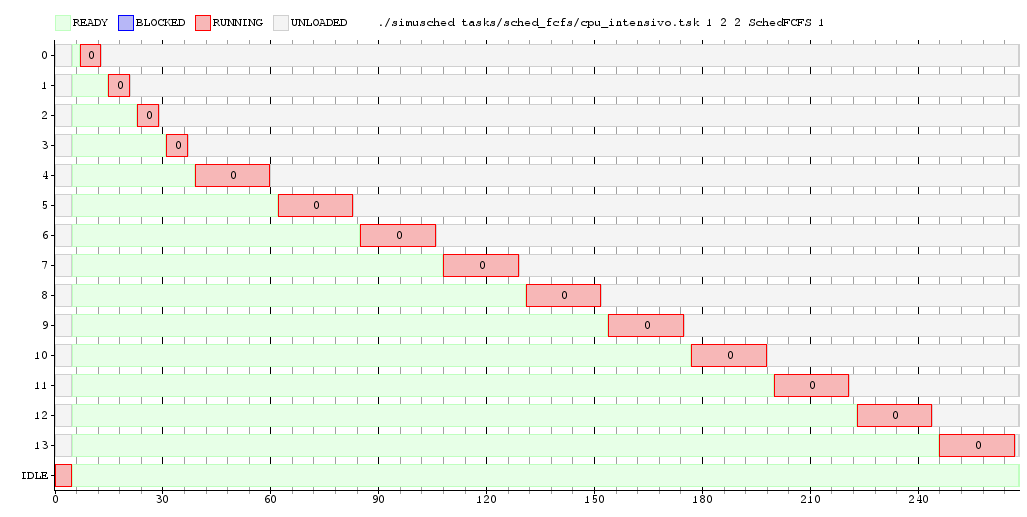
\includegraphics [width=\textwidth]{../graficos/sched_fcfs/cpu_intensivo.png}
  \caption{Intensivas en CPU}
\end{figure}
\begin{figure}[H]
  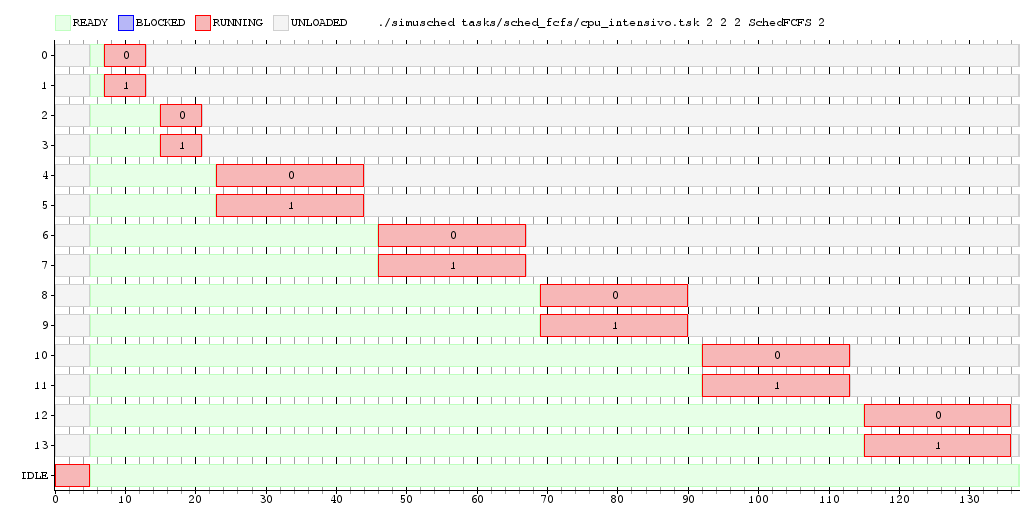
\includegraphics [width=\textwidth]{../graficos/sched_fcfs/cpu_intensivo2.png}
  \caption{Intensivas en CPU}
  \label{fig:intensivas-2cpu}
\end{figure}
\begin{figure}[H]
  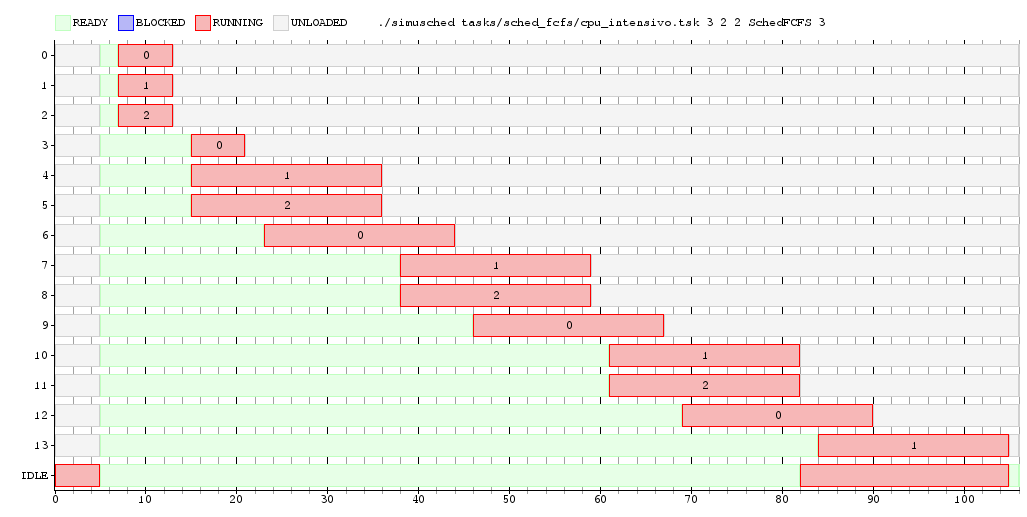
\includegraphics [width=\textwidth]{../graficos/sched_fcfs/cpu_intensivo3.png}
  \caption{Intensivas en CPU}
\end{figure}
\begin{figure}[H]
  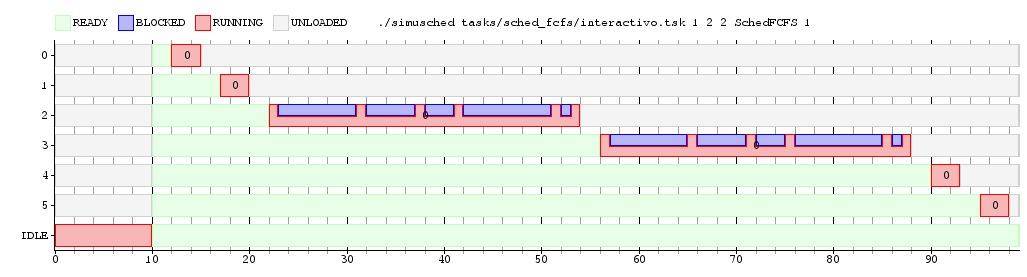
\includegraphics [width=\textwidth]{../graficos/sched_fcfs/interactivo.png}
  \caption{Interactivas}
\end{figure}
\begin{figure}[H]
  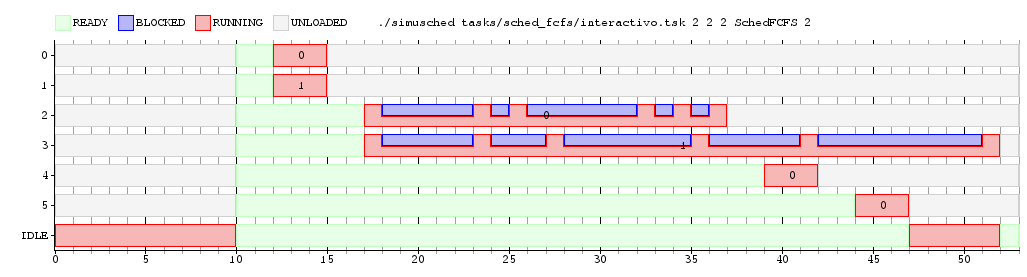
\includegraphics [width=\textwidth]{../graficos/sched_fcfs/interactivo_2.png}
  \caption{Interactivas}
\end{figure}
\begin{figure}[H]
  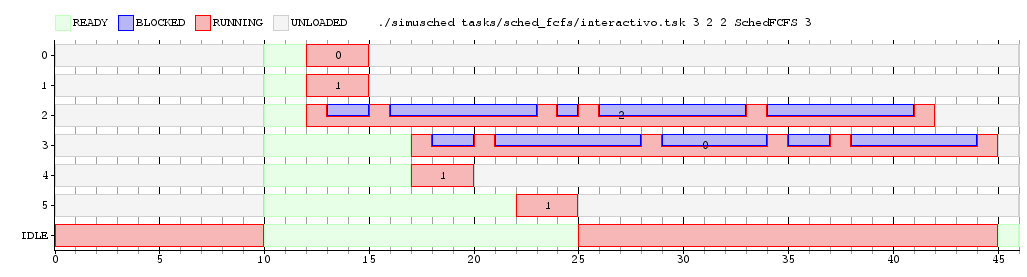
\includegraphics [width=\textwidth]{../graficos/sched_fcfs/interactivo_3.png}
  \caption{Interactivas}
\end{figure}
\begin{figure}[H]
  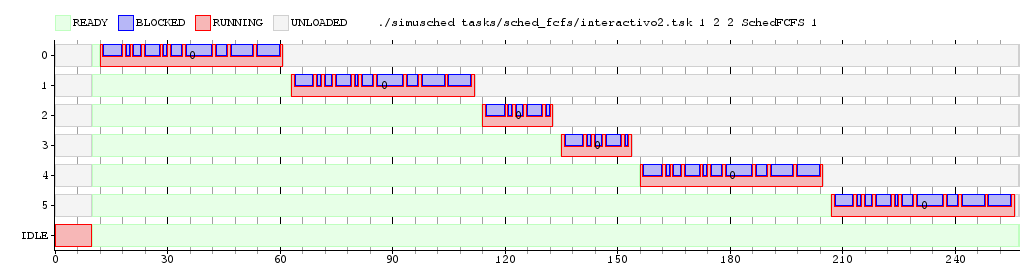
\includegraphics [width=\textwidth]{../graficos/sched_fcfs/interactivo2.png}
  \caption{Interactivas (2)}
\end{figure}
\begin{figure}[H]
  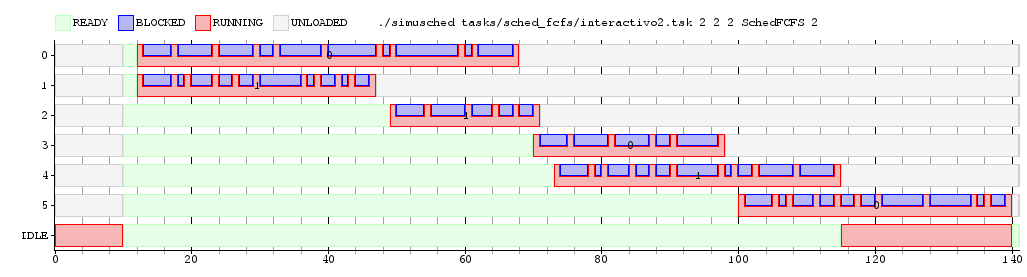
\includegraphics [width=\textwidth]{../graficos/sched_fcfs/interactivo2_2.png}
  \caption{Interactivas (2)}
\end{figure}
\begin{figure}[H]
  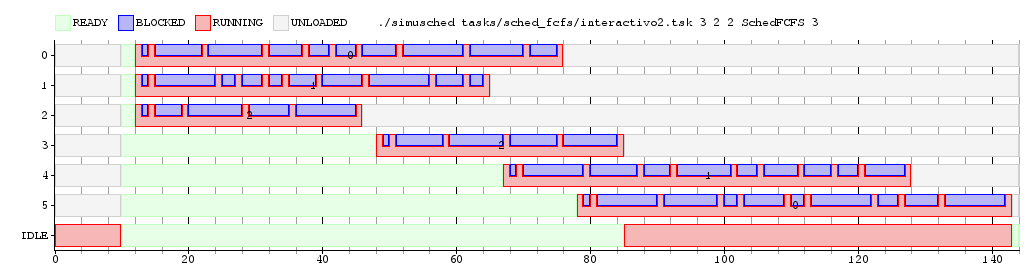
\includegraphics [width=\textwidth]{../graficos/sched_fcfs/interactivo2_3.png}
  \caption{Interactivas (2)}
\end{figure}

\clearpage





\index{Extendiendo el simulador con nuevos schedulers}
\section{Extendiendo el simulador con nuevos schedulers}
\setcounter{subsection}{2}

\subsection{Ejercicio 3}
Ahora pasaremos a explicar algunos aspectos relevantes de la implementación que hicimos del shceduler
$Round-Robin$, cuya idea básica es asignar espacios de tiempo equitativos a cada proceso y ir pasando
de uno a otro en forma circular, sin asignar ningún tipo de prioridad a ningún proceso. Una
característica interesante de este sistema de scheduling es que nos aseguramos de no tener el problema
conocido como $starvation$. 

En la implementación, recibimos como parámetro la cantidad de núcleos con la que vamos a trabajar
y los valores de sus respectivos $quantums$. Utilizamos una única cola global, para permitir así la
migración de proceso entre núcleos. La clase SchedRR consta de una parte pública y una privada. En 
la pública, se cuenta (al igual que en SchedLottery) con las funciones $load(pid)$, $unblock(pid)$ 
y $tick(cpu, motivo)$. La función de load es la de notificar al scheduler que un nuevo proceso ha llegado.
Cada vez que esto sucede, agregamos a la cola de procesos el pid del de dicho proceso. Unblock se encarga 
de que en la próxima llamada a la función tick, el proceso pid esté disponible para ejecutar. Y 
finalmente, tick se encarga de manejar, de acuerdo a qué fue lo último que hizo el proceso antes de llamar
a dicha función y a la porción del $quantum$ ya utilizado por el proceso, de encolar en la cola de procesos
al proceso actual y pasar a correr el próximo proceso si ya se utilizó todo el $quantum$, de pasar a correr 
el próximo proceso y dejar fuera de la lista de procesos al proceso actual si dicho proceso ha finalizado, o de
poner a correr el próximo proceso y encolar en la lista de procesos al proceso actual si dicho proceso se ha
bloqueado por alguna razón. 

Por otro lado, esta la parte privada de la clase SchedRR. Consta de algunas variables que utilizamos para efectuar
correctamente el manejo de procesos según la plítica del round-robin. Usamos un $vector<int> cores\_ticks$, 
con el que llevamos la cuenta en todo momento de la cantidad de ticks que consumió el proceso actual, 
para cada núcleo. También utilizamos un $vector<int> cores\_quantums$, en el cuál almacenamos los quantums
de cada procesador que nos son pasados por parámetro. Otra estructura de datos importante es una
$queue<int> process\_queue$, en la cuál almacenamos todos los procesos que están esperando a ser ejecutados.
En $cores_count$ guardamos la cantidad de núcleos con la que vamos a trabajar. Finalmente, implementamos la
función $run\_next(cpu)$, que devuelve el pid del próximo proceso de la cola a ejecutar. Sólo la invocamos
cuando es necesario pasar a ejecutar un nuevo proceso. Y lo que hacemos es sacar el primer proceso que está 
esperando en la cola de la misma y ponerlo a correr, al mismo tiempo que inicializamos la variable
$cant\_ticks[pid]$ a cero (inicializamos el contador de ticks para el proceso actual en ejecución a cero). 









\clearpage
\subsection{Ejercicio 4}

Para este ejercicio se pide diseñar lotes de tareas, y luego simularlos mediante
el Scheduler \texttt{SchedRR} implementado en el \textbf{punto 3}. Se diseñó un
lote de \textbf{tareas  simples}\footnote{Solo usan CPU.}, y tres lotes
conteniendo \textbf{tareas simples} y  \textbf{tareas interactivas} con
distintos criterios de orden. Se corrió el  experimento con \texttt{1 CPU}, y
con \texttt{2 CPU}, con un \emph{Quantum} de 2.

\begin{minipage}[t]{0.4\textwidth}
\begin{Verbatim}[frame=single,framesep=1cm,label=simples.tsk]
*10 TaskCPU 5  
\end{Verbatim}
\end{minipage}
\hfill
\begin{minipage}[t]{0.4\textwidth}
\begin{Verbatim}[frame=single,framesep=1cm,label=interactivas.tsk]
*6 TaskCPU 6
*6 TaskConsola 6 1 12
\end{Verbatim}
\end{minipage}

\begin{minipage}{0.4\textwidth}
\begin{Verbatim}[frame=single,framesep=1cm,label=interactivas2.tsk]
*6 TaskConsola 6 1 12
*6 TaskCPU 6
\end{Verbatim}
\end{minipage}
\hfill
\begin{minipage}{0.4\textwidth}
\begin{Verbatim}[frame=single,framesep=1cm,label=interactivas\_intercaladas.tsk]
TaskCPU 6
TaskConsola 6 1 12
TaskCPU 6
TaskConsola 6 1 12
TaskCPU 6
TaskConsola 6 1 12
TaskCPU 6
TaskConsola 6 1 12
TaskCPU 6
TaskConsola 6 1 12
\end{Verbatim}
\end{minipage}

En el lote de \textbf{tareas simples}, estas comienzan al mismo tiempo, y  son
ejecutadas con los mismos parámetros, de forma tal que tanto en la simulación
con \texttt{1 core} como en la de \texttt{2 cores} es fácil visualizar el
comportamiento característico del \textbf{Round Robin}. Esto se puede apreciar
en \fig{gantt-sched-rr-1} y \fig{gantt-sched-rr-2}, de uno y dos \textbf{cores}
respectivamente.  En ambas versiones se puede notar que en ningún momento hay un
``desperdicio'' de CPU, pero dado que no hay llamadas bloqueantes esto es de
esperarse. Por la misma razón, también es más notorio el orden en que son
llamadas las tareas, ya que como estas jamás se bloquean, siempre están
disponibles apenas terminan su \emph{Quantum}. En la versión de \textbf{2 cores}
se puede observar, además, que no se realiza migración de procesos entre
núcleos, ya que el número de tareas es par. Si el número de tareas fuera impar,
esto obligaría a todas las tareas a migrar de núcleo.

\begin{figure}
  \centering
  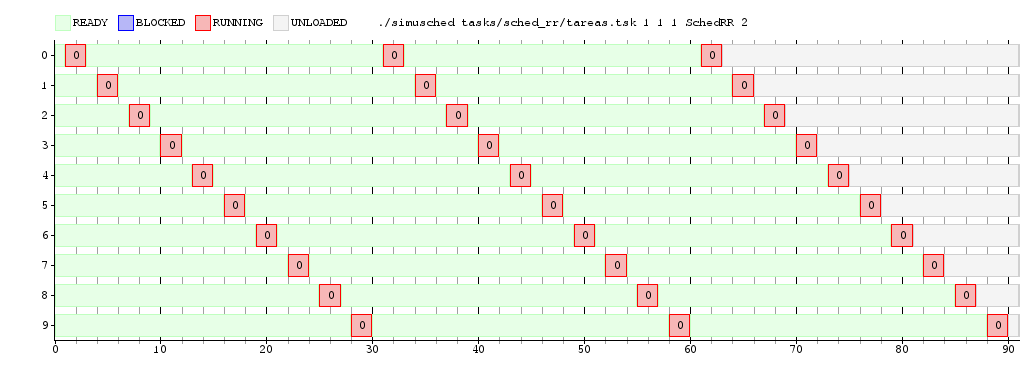
\includegraphics [width=\textwidth]{../graficos/sched_rr/simples-1.png}
  \caption{\emph{Diagrama Gantt} de \texttt{SchedRR} para tareas simples \textbf{(1 core)}}
  \label{fig:gantt-sched-rr-1}
\end{figure}

\begin{figure}
  \centering
  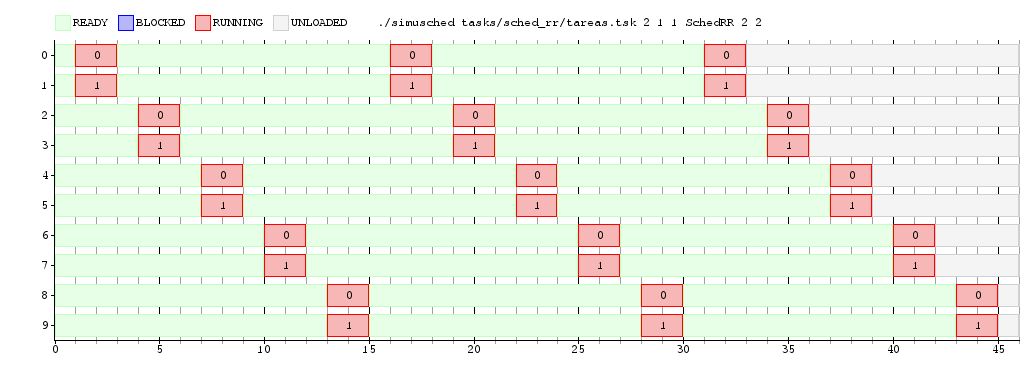
\includegraphics [width=\textwidth]{../graficos/sched_rr/simples-2.png}
  \caption{\emph{Diagrama Gantt} de \texttt{SchedRR} para tareas simples \textbf{(2 cores)}}
  \label{fig:gantt-sched-rr-2}
\end{figure}

Los lotes de \textbf{tareas interactivas} producen resultados más interesantes.
Para probar las diferentes opciones se varió el orden de las tareas. En \fig
{gantt-sched-rr-interactivas1-1} y \fig{gantt-sched-rr-interactivas1-2} se
pueden observar los diagramas correspondientes a las versiones de 1 core y 2
cores, para los lotes en donde se encolan primero las \textbf{6 tareas simples},
y luego las \textbf{6 tareas interactivas}. En la versión de \textbf{1 core},
vemos que no hay \emph{desperdicio de CPU}. Sin embargo, en la versión de
\textbf{2 cores}, se puede observar que la \textbf{tarea IDLE} corre varias
veces, durante una cantidad considerable de ciclos, luego de que todas las
\textbf{tareas simples} ya terminaron su ejecución. Esto coincide con los
momentos en que todas las \textbf{tareas interactivas} se encuentran
\emph{bloqueadas}. También podemos notar que, aunque en la segunda versión el
número de cores es el doble, el tiempo de ejecución total de todas las tareas no
es la mitad que para la primera versión.

En \fig{gantt-sched-rr-interactivas2-1} y \fig{gantt-sched-rr-interactivas2-2}
se pueden observar los diagramas correspondientes a las versiones de 1 core y 2
cores, para los lotes en donde se encolan primero las \textbf{6 tareas
interactivas}, y luego las \textbf{6 tareas simples}. Pese al cambio de orden,
se sigue notando el mismo tipo de patrón, característico de una planificación
por \textbf{Round Robin}. En la versión de \textbf{2 cores} se nota una leve
mejoría con respecto a la versión de \fig{gantt-sched-rr-interactivas1-2}, a
causa de un mejor aprovechamiento de la CPU: como las \textbf{tareas
interactivas} fueron encoladas primero, se le está dando una pequeña
``ventaja/prioridad'' frente a las \textbf{tareas simples}. Esto permite que
cuando las primeras se bloquean, las segundas \emph{aprovechen el tiempo de
CPU} libre, evitando delegárselo a la \textbf{tarea IDLE}.

Finalmente, en \fig{gantt-sched-rr-interactivas-interrcaladas-1} y  
\fig{gantt-sched-rr-interactivas-interrcaladas-2} también se puede apreciar 
fácilmente el comportamiento de la \emph{planificación Round Robin}. Las tareas
se encuentran intercaladas, buscando así forzar una distribución más equitativa
entre las \textbf{tareas interactivas} y las \textbf{tareas no interactivas}. En
la versión de \textbf{1 core}, se puede notar rápidamente cómo el orden inicial
se va perdiendo, relegando la ejecución de las \textbf{tareas bloqueantes}. Esto
último se observa todavía más acentuado en la versión de \textbf{2 cores}, en
donde además hay una alta tasa de migración de CPU. A pesar de ello, las
\textbf{tareas no interactivas} tienen un tiempo total de ejecución levemente
superior a \fig{gantt-sched-rr-interactivas1-2}, en donde estas son puestas al
principio de la cola.

\begin{figure}
  \centering
  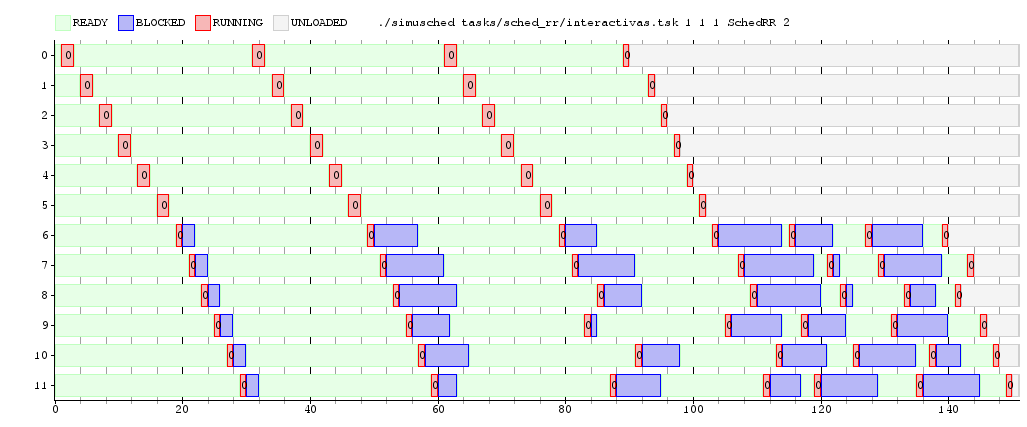
\includegraphics [width=\textwidth]{../graficos/sched_rr/interactivas1-1.png}
  \caption{\emph{Diagrama Gantt} de \texttt{SchedRR} para tareas simples, luego interactivas \textbf{(1 core)}}
  \label{fig:gantt-sched-rr-interactivas1-1}
\end{figure}

\begin{figure}
  \centering
  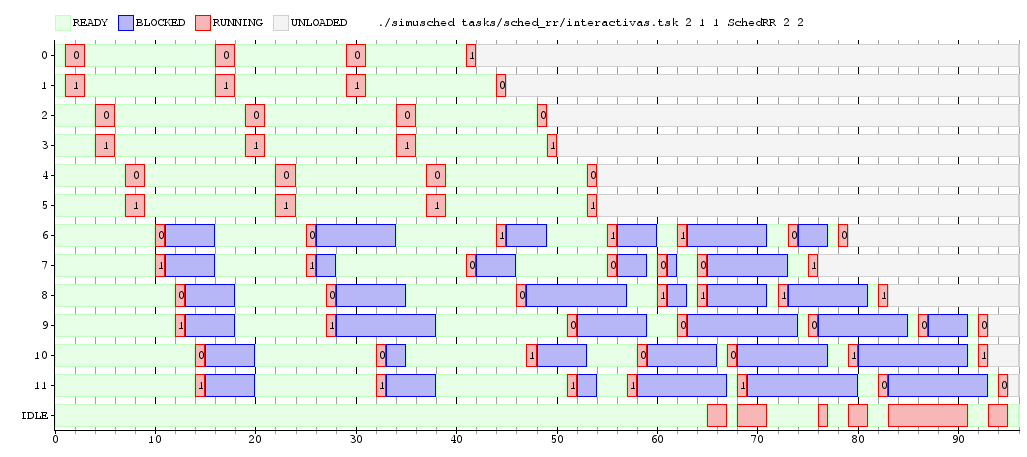
\includegraphics [width=\textwidth]{../graficos/sched_rr/interactivas1-2.png}
  \caption{\emph{Diagrama Gantt} de \texttt{SchedRR} para tareas simples, luego interactivas \textbf{(2 cores)}}
  \label{fig:gantt-sched-rr-interactivas1-2}
\end{figure}

\begin{figure}
  \centering
  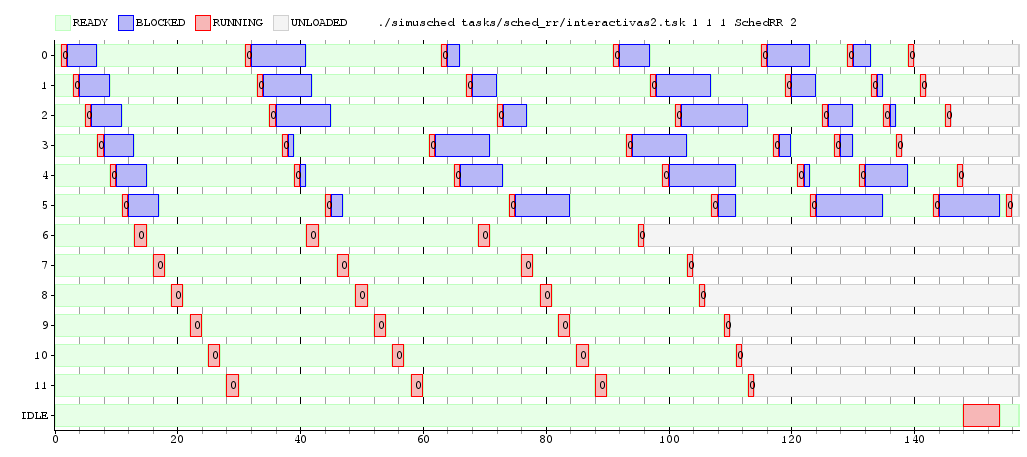
\includegraphics [width=\textwidth]{../graficos/sched_rr/interactivas2-1.png}
  \caption{\emph{Diagrama Gantt} de \texttt{SchedRR} para tareas interactivas, luego simples \textbf{(1 core)}}
  \label{fig:gantt-sched-rr-interactivas2-1}
\end{figure}

\begin{figure}
  \centering
  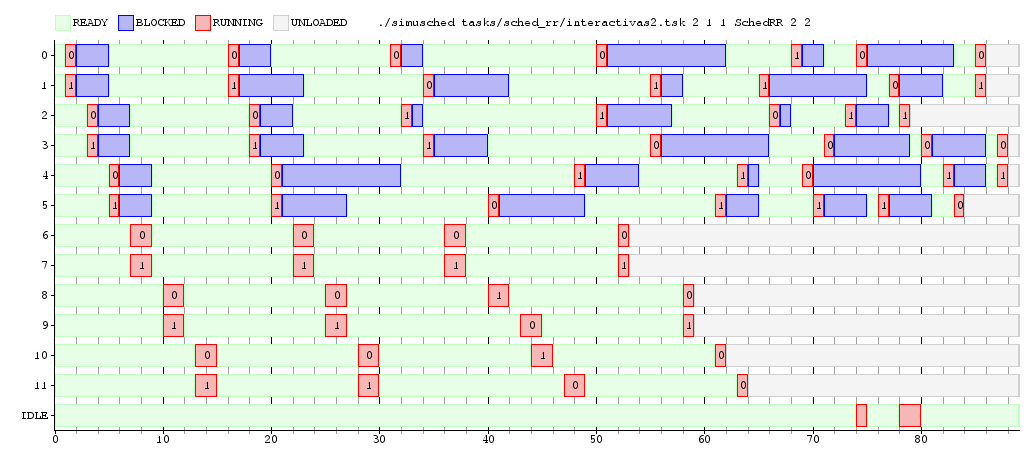
\includegraphics [width=\textwidth]{../graficos/sched_rr/interactivas2-2.png}
  \caption{\emph{Diagrama Gantt} de \texttt{SchedRR} para tareas interactivas, luego simples \textbf{(2 cores)}}
  \label{fig:gantt-sched-rr-interactivas2-2}
\end{figure}

\begin{figure}
  \centering
  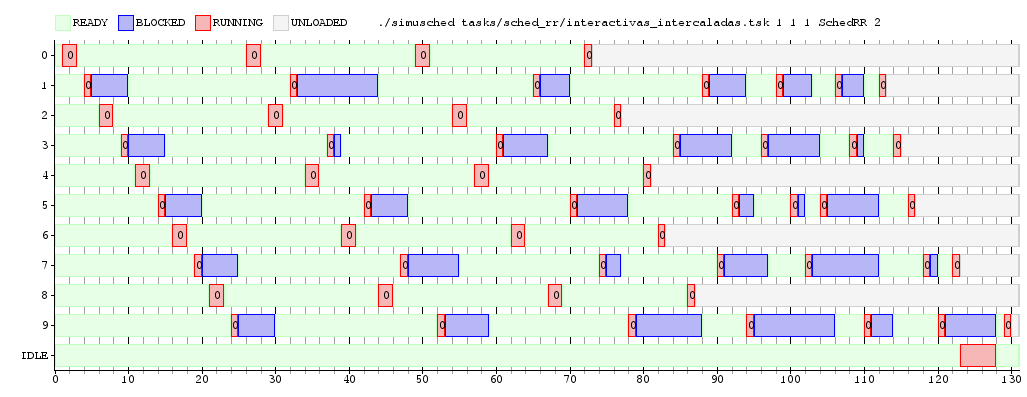
\includegraphics [width=\textwidth]{../graficos/sched_rr/interactivas-intercaladas-1.png}
  \caption{\emph{Diagrama Gantt} de \texttt{SchedRR} para tareas simples e interactivas, intercaladas \textbf{(1 core)}}
  \label{fig:gantt-sched-rr-interactivas-interrcaladas-1}
\end{figure}

\begin{figure}
  \centering
  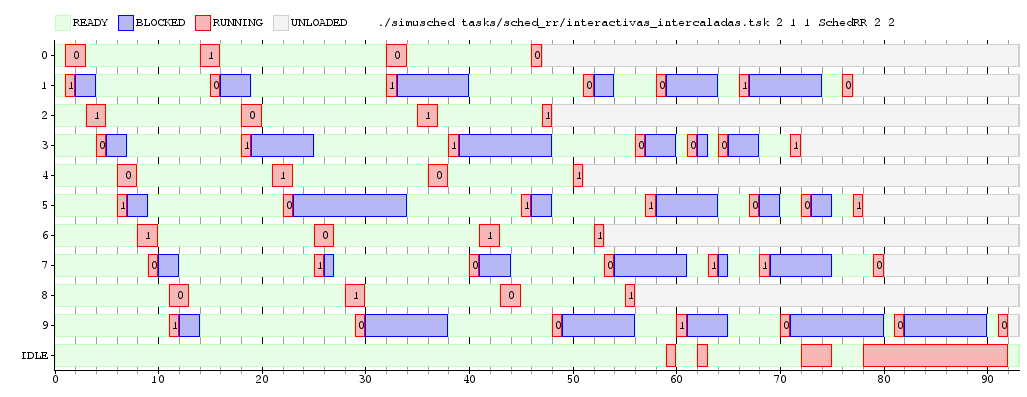
\includegraphics [width=\textwidth]{../graficos/sched_rr/interactivas-intercaladas-2.png}
  \caption{\emph{Diagrama Gantt} de \texttt{SchedRR} para tareas simples e interactivas, intercaladas \textbf{(2 cores)}}
  \label{fig:gantt-sched-rr-interactivas-interrcaladas-2}
\end{figure}



\clearpage
\subsection{Ejercicio 5}
En este ejercicio, basados en el paper de Waldspurger, C.A. y Weihl en el cuál presentan un 
novedoso sistema de Scheduling llamado $Lottery Scheduling$, implementamos una clase que llamamos
SchedLottery que recibe como parámetros el quantum que se va simular y una semilla 
pseudo-aleatoria, que el scheduler va a utilizar para el manejo de los procesos. Como dice en el
enunciado, básicamente nos interesó implementar la idea básica del algoritmo y la 
optimización de tickets compensatorios y en este caso, siempre trabajamos sólo con un núcleo. 

La clase SchedLottery tiene como parte pública las funciones \texttt{load(pid)}, \texttt{unblock(pid)} 
y \texttt{tick(cpu, motivo)}. 

i) La función load(pid) la utilizamos para notificar al scheduler
que un nuevo proceso ha llegado. Cada vez que llega un nuevo proceso le damos un ticket a dicho proceso.
De esta forma, en el próximo sorteo el proceso será candidato a ganarlo y así ser el próximo 
en ser ejecutado. 

ii) La función
tick(cpu, motivo). El parámetro motivo puede significar que una de tres cosas
ocurrieron durante el último ciclo del reloj: la tarea pid consumió todo su
ciclo utilizando el CPU número $cpu$ (en cuyo caso incrementamos la cantidad de ticks y si esta cantidad supera el
quantum de dicho procesador, la desalojamos), la tarea ejecutó una llamada bloqueante o permaneció 
bloqueada durante el último ciclo (en cuyo caso proveemos al proceso bloqueado la compensación 
de tickets correspondiente basándonos en el paper antes mencionado) ó porque la tarea pid 
terminó (en cuyo caso desalojamos la tarea
actual). Después de hacer estos chequeos, corremos \texttt{run\_lottery()} que se encarga de efectuar el 
sorteo de tickets para la próxima vez que se necesite elegir un proceso ganador y así asignarle 
los recursos necesarios. 

iii) La función unblock(pid) hace que en la próxima llamada a la función tick, el proceso pid 
esté disponible para ejecutar. Lo que hacemos, es entregarle al proceso pid la cantidad de tickets
que tenía el proceso antes de ser bloqueado multiplicado por la compensación correspondiente, que 
depende de qué fracción del quantum dicho proceso hizo del CPU. 

Por otro lado, la clase SchedLottery tiene una parte privada, que consta de variables como $quantum$, 
que usamos para saber el quantum que tiene disponible cada proceso para ejecutarse, $seed$, que
usamos como semilla para elegir el ticket ganador cada vez que hagamos un sorteo, $vector<ticket>$, que
usamos para saber qué tickets corresponden a cada proceso, $total\_tickets$ para tener rápido acceso
a la cantidad de tickets que hay distribuidos entre los procesos y $tick\_number$ que usamos para 
llevar la cuenta de cuántas veces llamamos a la función tick(cpu,motivo). Además, contamos con 
las funciones privadas $compensa(pid)$, $desaloja(pid)$ y $tickets\_index(pid)$. La primera se encarga de
calcular y asignar la compensación deseada a un proceso cuando corresponda; la segunda de que cuando
se bloquea un proceso, no esté disponible para ejecutar en la próxima ejecución de la función
tick(cpu,motivo). Es decir, que la probabilidad de ser elegible en el sorteo sobre los tickets sea cero.
Para eso, lo que hicimos fue sacarle todos los tickets temporalmente a dicho proceso. 






\clearpage
\index{Evaluando los algoritmos de scheduling}
\section{Evaluando los algoritmos de scheduling}
\setcounter{subsection}{5}






\subsection{Ejercicio 6}

Se registró un nuevo tipo de tarea, \texttt{TaskBatch(total\_cpu, cant\_bloqueos)}. Hace uso del CPU $total\_cpu$ ticks de reloj en total, entre los cuáles hace $cant\_bloqueos$ llamadas bloqueantes, distribuidas de manera uniforme y de duración un tick de reloj.
La implementación requirió elegir $cant\_bloqueos$ momentos entre 1 y $total\_cpu$. Para eso se guardó un arreglo de booleanos que mantiene que momentos ya fueron elegidos. Entonces se fueron generando momentos de manera pseudo\-aleatoria hasta elegir $cant\_bloqueos$ momentos \textit{distintos} para hacer llamadas bloqueantes. En el resto del tiempo, la tarea usa el procesador.







\clearpage
\subsection{Ejercicio 7}
En este ejercicio, el objetivo es definir dos m\'etricas diferentes y a partir de estas y variando la
cantidad de n\'ucleos utilizados y para distintos $quantums$,  concluir cu\'al es el valor \'optimo de 
$quantum$ a los efectos de las distintas m\'etricas. \\
La primera m\'etrica interesante que se nos ocurri\'o fue la de considerar la mediana de los tiempos extra
que se demoraron cada uno de los procesos en finalizar, de acuerdo al tiempo m\'inimo que cada uno de dichos 
procesos se demorar\'ia en terminar si fueran corridos cada uno por un \'unico procesador. Como se pide en
el enunciado, mantuvimos fijo en 1 el ciclo de reloj y el costo de cambio de contexto y 2 los ciclos de 
migraci\'on entre n\'ucleos.

Analizamos qu\'e sucede cuando empleamos uno y cuatro n\'ucleos. El valor 
\'optimo de $quantum$ para esta m\'etrica depender\'a, por ejemplo, de si lo que queremos es maximizar 
ecuanimidad en la ejecuci\'on de procesos o de si queremos minimizar el tiempo de ejecuci\'on de cada
proceso. En el primer caso, elegir\'iamos un $quantum$ tal que el gr\'afico de tiempo residual de ejecuci\'on
en funci\'on del quantum sea lo m\'as parecido a una constante. 

En estos gráficos, pretendemos representar
para cada quantum, la mediana de todos los tiempos residuales de ejecución, junto con el mínimo
y el máximo tiempo residual. Podemos analizar las tres curvas que quedan asi formadas: si la curva de la 
mediana está a corta distancia de, por ejemplo, la curva de máximos, entonces esto nos indicaría
que la mayor parte de los procesos tienen un tiempo residual de ejecución grande, mientras que si
estuviera cerca de la curva mínima, entonces la mayor parte de los procesos tienen un tiempo residual de 
ejecución pequeño. 

\begin{figure}[H]
  \centering
  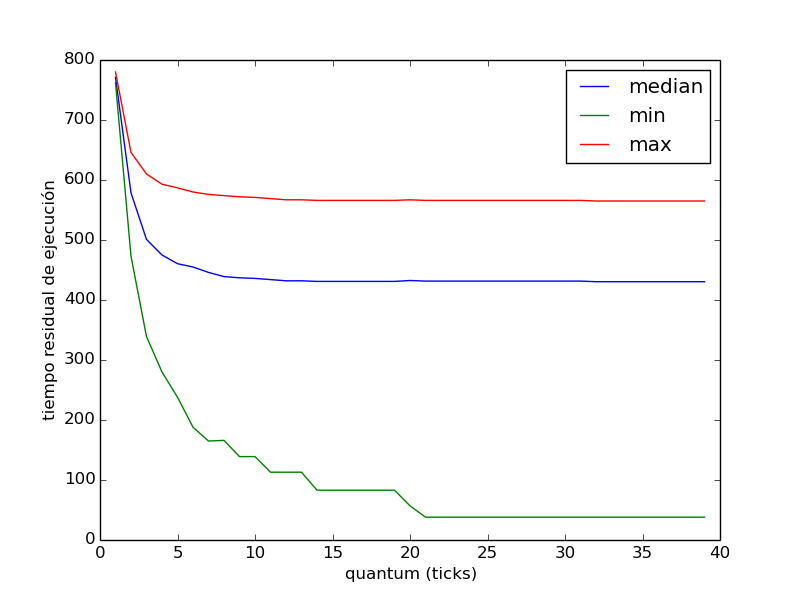
\includegraphics [width=\textwidth]{../graficos/metrica_eze_plot_batch_1core_fidedigno.png}
  \caption{\emph{Métrica 1}: tiempo residual \textbf{(1 core)}}
  \label{fig:eze-1core}
\end{figure}

Además, el valor para el cuál se estabiliza la curva de medianas nos dará la pauta de en qué rango se encuentra
el quantum  óptimo que podemos tomar para minimizar (usando cierta cantidad de cores) el tiempo residual 
de ejecución de los procesos. 

Teniendo todo esto en cuenta, consideramos que en \fig{eze-1core} el quantum óptimo se encuentra entre 5 y 10.
No tomamos un quantum mayor ya que no percibimos ningún tipo de ventaja en tomar un valor que podría
perjudicar la calidad del scheduler desde la perspectiva de otras métricas (como ecuanimidad, ya que al 
ampliar el quantum estamos ampliando de igual forma la heterogeneidad en la distribución del tiempo de CPU),
sin aportar ningún tipo de beneficio apreciable a los efectos de esta.
Con \fig{eze-4core} sucede algo similar, con dos diferencias básicas: la primera es que las tres funciones
graficadas son menores, y que la media se encuentra, en proporción, más cerca del
mínimo que con un sólo core. Y dado que la mitad de los valores se encuentran debajo de la media, podemos
afirmar que en líneas generales la mayoría de los valores resultan ser mucho menores. Otro detalle
a considerar, son las pequeñas variaciones en las curvas, que no se dan en el caso de 1 core. Estas ocurren
debido a que al hacer uso de más de 1 core, la probabilidad de que ocurra el evento ``todas las tareas
se encuentran bloqueadas'' es mucho más alta.

Observamos que con quantums muy pequeños, el tiempo residual de ejecución es casi el doble que el percibido
con un quantum óptimo. Adjudicamos estos valores a la similitud entre los valores del quantum y los tiempos 
de migración y cambio de contexto; bajo estas circunstancias, gran parte del tiempo de CPU es utilizado para
realizar estas tareas. Se puede apreciar también que el nivel de ecuanimidad (fairness) crece a medida que 
el quantum disminuye (porque las curvas se acercan unas a otras), sin embargo no es un beneficio 
considerable frente al gran aumento del tiempo residual. 

\begin{figure}[H]
  \centering
  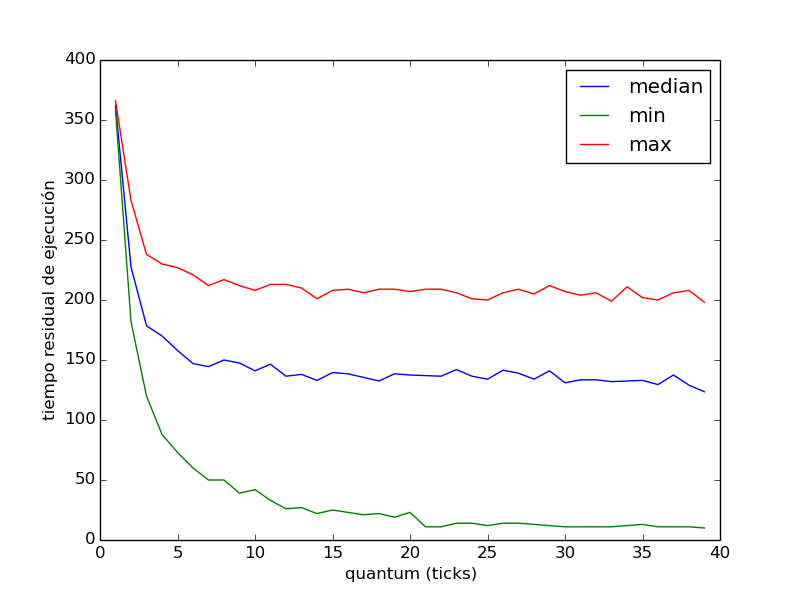
\includegraphics [width=\textwidth]{../graficos/metrica_eze_plot_batch_4core.png}
  \caption{\emph{Métrica 1}: tiempo residual \textbf{(4 cores)}}
  \label{fig:eze-4core}
\end{figure}

La segunda métrica que consideramos fue el tiempo de respuesta, que esta definido como el tiempo que 
transcurre entre que una tarea se desbloquea y vuelve a tomar el control del procesador. Para cada proceso,
calculamos la mediana de los tiempos de respuesta en cada llamada bloqueante. De entre ellos, tomamos 
para cada quantum, los valores máximo, mínimo y mediano. Así obtuvimos \fig{metrica-gonza-1core} para las 
mediciones efectuadas con un único core y \fig{metrica-gonza-4cores} para las mediciones efectuadas con cuatro
cores. 

\begin{figure}
  \centering
  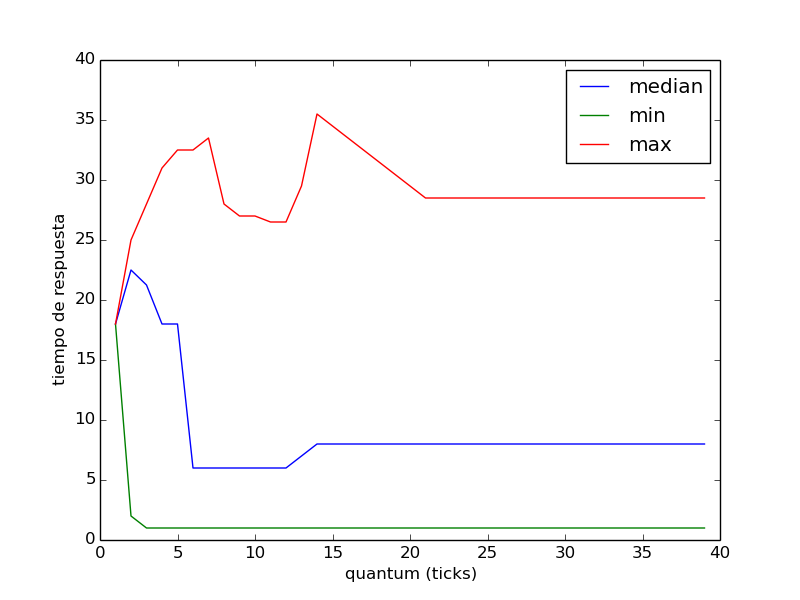
\includegraphics [width=\textwidth]{../codigo/plot-respuesta-muybueno.png}
  \caption{\emph{Métrica 2}: tiempo de respuesta \textbf{(1 core)}}
  \label{fig:metrica-gonza-1core}
\end{figure}

\begin{figure}
  \centering
  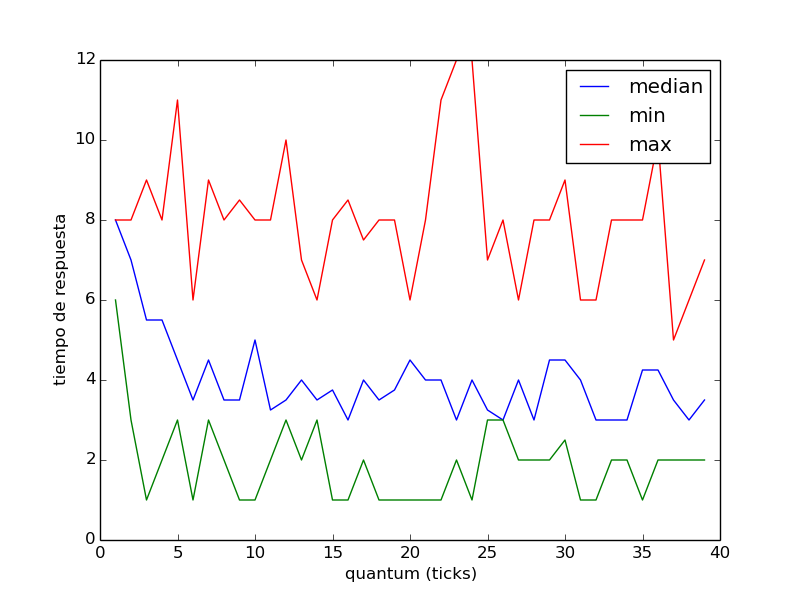
\includegraphics [width=\textwidth]{../codigo/plot-respuesta-4core-unpocomejor.png}
  \caption{\emph{Métrica 2}: tiempo de respuesta \textbf{(4 cores)}}
  \label{fig:metrica-gonza-4cores}
\end{figure}

En \fig{metrica-gonza-1core} se puede observar un mínimo local entre los valores 6 y 14 de quantum. Este 
mínimo no es muy pronunciado, y al igual que para la métrica anterior, hay un valor de quantum a partir
del cuál el tiempo de respuesta (antes era el tiempo residual) se estabiliza. En este caso tomamos como
quantum óptimo el valor 10. 

En \fig{metrica-gonza-4cores} se observan tres curvas que presentan una gran fluctuación y no se puede 
encontrar un valor de quantum óptimo ó uno a partir del cuál el tiempo de respuesta se estabilize. De todas 
formas, por más que hay una fluctuación marcada en los tiempos de respuesta, este varía en el mismo rango
aproximadamente (entre 3 y 4) a partir de un cierto valor de quantum (quantum = 5). 

Algo muy destacable de esta métrica, en comparación con la anterior, es que su media está posicionada más
cerca del valor mínimo que del valor máximo (algo que no sucedía en la primera métrica).



\clearpage
\subsection{Ejercicio 8}
En esta sección implementamos una segunda versión para el scheduler tipo $Round-Robin$ que ya implementamos
en ejercicios anteriores. En este caso, el objetivo es no permitir la migración de procesos entre núcleos y
analizar qué sucede con la performance de este scheduler en comparación con el original para distintos lotes
de tareas. En principio, esperaríamos que en algunos tipos de lotes un algoritmo ande mejor que el otro.

Un ejemplo fácil de ver en donde el Scheduler sin migración tiene una performance menor a la del anterior,
es cuando se cuenta con uno o más procesos de mucha duración, alojados en un mismo núcleo, y muchos procesos
pequeños alojados en el resto de los nucleos. En este escenario, los procesos pequeños terminarían rápidamente,
liberando sus respectivos núcleos, mientras que los otros estarían obligados a correr en su núcleo original, 
sin la posibilidad de migrar a los núcleos disponibles. 

Basandonos en las ideas anteriores, realizamos una experimentación en donde buscamos
explotar esta debilidad. La misma se puede apreciar en \fig{ej8-1} y \fig{ej8-2}. Sabiendo
el código interno de asignación de procesos a la CPU, pudimos recrear un lote de tareas, compuesto
por 3 tareas ``grandes'' y 8 tareas ``pequeñas'', de forma tal que el orden de las mismas ocasionase 
que todas las tareas grandes caigan en un mismo procesador. En poco tiempo, todas las tareas pequeñas
terminan su ejecución, liberando el resto de los núcleos. Aquí, se puede notar la gran ventaja del
\textbf{Scheduler Round Robin con migración}, ya que en este punto las tres tareas restantes se 
ejecutan de forma paralela, terminando la ejecución de todas las tareas aproximadamente a los 
130 ciclos de clock. En la versión \textbf{sin migración}, en cambio, las tres tareas se ejecutan
secuencialmente, casi-triplicando el tiempo total de ejecución, sobrepasando los 330 clocks totales.
A continuación se puede apreciar la entrada utilizada para generar los gráficos:

\begin{center}
\begin{minipage}{0.4\textwidth}
\begin{Verbatim}[frame=single,framesep=1cm,label=ej8.tsk]
@1:
TaskCPU 100
@2:
TaskCPU 10
@3:
TaskCPU 10
@4:
TaskCPU 10
@5:
TaskCPU 10
@6:
TaskCPU 100
@7:
TaskCPU 10
@8:
TaskCPU 10
@9:
TaskCPU 10
@10:
TaskCPU 10
@11:
TaskCPU 100
\end{Verbatim}
\end{minipage}
\end{center}

\begin{figure}[H]
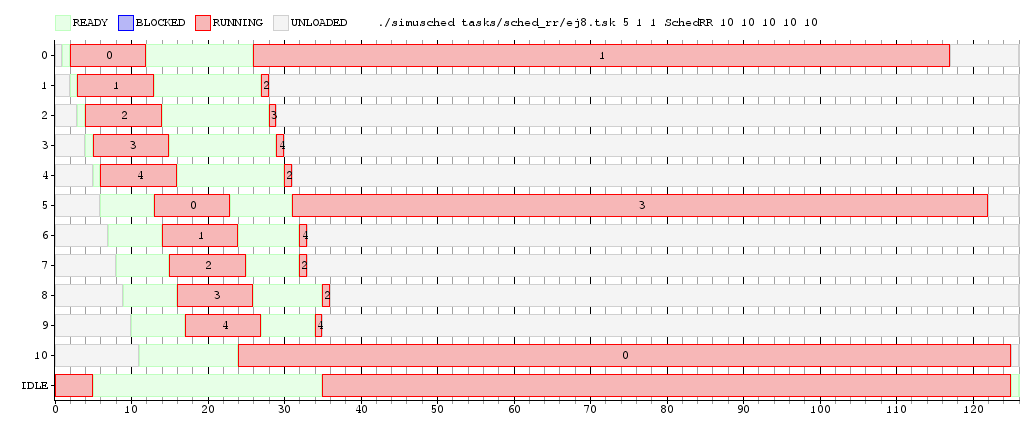
\includegraphics [width=\textwidth]{../graficos/sched_rr/ej8-sched-rr.png}
\caption{Diagrama de Gantt SchedRR}
\label{fig:ej8-1}
\end{figure}
\begin{figure}[H]
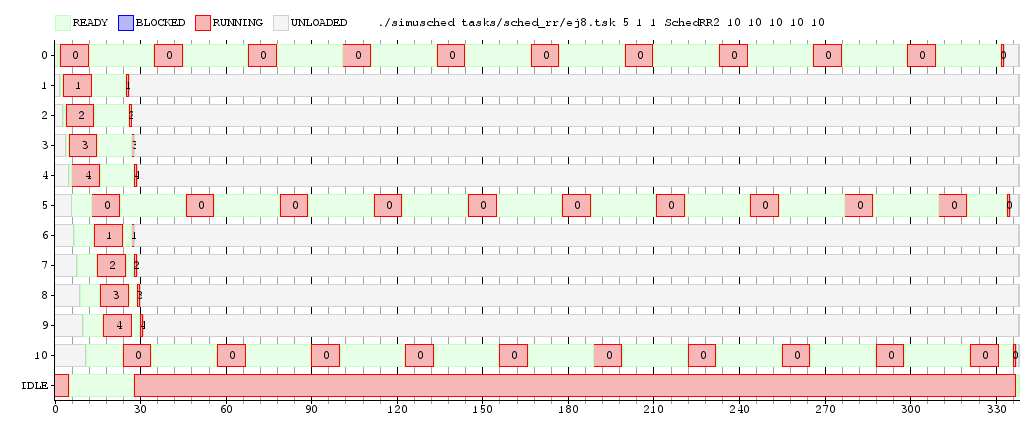
\includegraphics [width=\textwidth]{../graficos/sched_rr/ej8-sched-rr2.png}
\caption{Diagrama de Gantt SchedRR2}
\label{fig:ej8-2}
\end{figure}

Finalmente, en principio creemos que si hubieran muchos más procesos que núcleos y de longitud similar, 
y no se permitiera la migración de procesos entre núcleos, los tiempos de finalización de distintos 
procesos serían muy dispares. Algo que, en principio es indeseable pues podría suceder que si a un proceso muy 
corto le toca justo el mismo core que a un proceso muy largo, este debería esperar mucho tiempo a que el largo
termine hasta que el procesador lo atienda. 

En nuestra implementación del la clase \texttt{SchedRR2},
para proveer las mismas tres funciones básicas que venimos
implementando en los anteriores schedulers (\textbf{TICK},\textbf{UNBLOCK},\textbf{LOAD}), 
utilizamos tres estructuras para el manejo de los procesos, estas son: 
un $vector<Core>$, que contiene para cada núcleo la información que teníamos 
en la implementación del $SchedRR$, y que era compartida por todos. En efecto, 
tenemos un \texttt{struct Core}, que almacena para cada procesador su quantum, la cantidad de 
ticks actual, un vector de enteros que lleva cuenta de los procesos activos en dicho núcleo, 
una cola de procesos que se encuentran disponibles (es decir, todos aquellos
que no se encuentren bloqueados), que permita saber en qué orden deben ser ejecutados.
Se implementó un método \texttt{runNextProcess(\textbf{CPU})}, que se encarga de preparar las estructuras
internas del scheduler para desalojar el proceso actual, y obtiene de la cola correspondiente a esa 
CPU el siguiente proceso.

Cuando se produce un UNBLOCK, simplemente encolamos el proceso nuevamente, en su CPU correspondiente. 
A través del método \textbf{getProcessCores(\texttt{pid})} obtenemos, dada la ID de un proceso,
un puntero a la CPU a la cual se encuentra asignado. Si el motivo de un tick es de \textbf{EXIT} 
o \textbf{BLOCK}, pasamos a correr al siguiente proceso, llamando al método, runNextProcess(). Si el
motivo del tick es \textbf{TICK}, comparamos el quantum del procesador con la cantidad de ticks actuales,
y si el mismo no resulta ser mayor, encolamos al proceso nuevamente, y luego llamamos a runNextProcess().

Al momento de hacer un \textbf{LOAD}, necesitamo saber en todo momento cual es la CPU que tiene menos
procesos activos. Para ello, utilizamos la función min\_element, que toma un elemento iterable, y un
\textbf{Operador de Comparación}, el cual es un \texttt{struct} que en su interior contiene la lógica
que le va a servir para deducir cuando, dados a y b dos Core, $a < b$. Esto se traduce, concretamente,
en la comparación de los tamaños de las listas de active-process de cada core, es decir 
$a.active\_process.size() < b.active\_process.size()$.



\clearpage
\subsection{Ejercicio 9}

Se procedió a analizar la ecuanimidad o $fairness$ de nuestra implementación de $Lottery\ Scheduler$.

Se eligieron cuatro procesos idénticos: $TaskCPU$ con 30 ticks de uso del procesador. Se lanzaron al mismo tiempo y se midió la cantidad de ticks que tomaron para finalizar la ejecución. Se esperaba que los cuatro procesos terminaran al mismo tiempo, si esperábamos un mecanismo de scheduling ecuánime.

Sin embargo, al correr el simulador distintos procesos terminaron en tiempos con hasta un 40\% de diferencia. Dado el carácter pseudoaleatorio de la elección del proceso a ejecutar, dada una corrida en particular no está garantizada una asignación equitativa de los recursos. Se extendió el experimento y se llegó a dos conclusiones importantes.

Primero, la ecuanimidad tiende a aumentar a medida que el tiempo aumenta. Se lanzaron 10 procesos idénticos al mismo tiempo, con un uso del CPU de 20 ticks, y un quantum de 4. Se fue midiendo, cada vez que se llama a \texttt{run\_lottery()} y se elige un proceso, la cantidad de ticks de procesador otorgados a cada proceso hasta el momento. Como medida de ecuanimidad se calculó la desviación estándar de estos valores.

A continuación se presentan los resultados.

\begin{figure}[H]
\centering
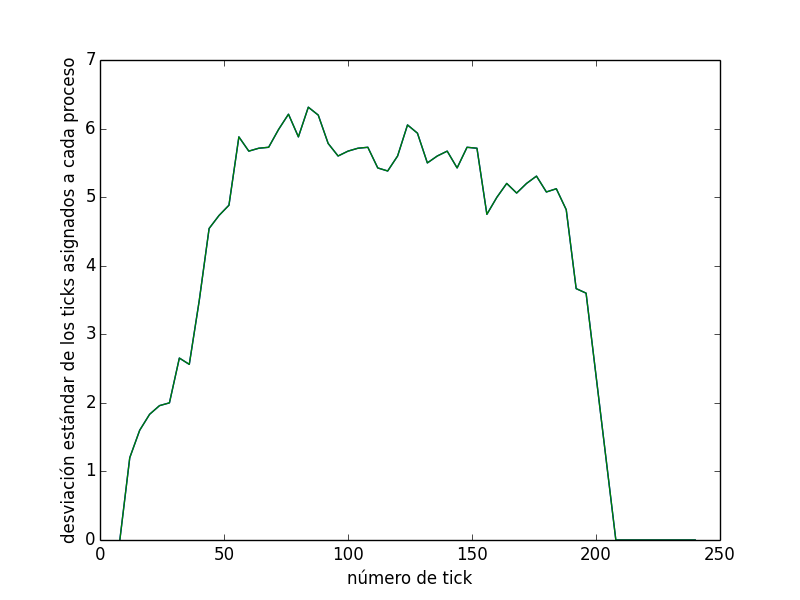
\includegraphics[width=\textwidth]{../experimentacion/ej9-fairness/fairness/plot.png}
\caption{Desvío estándar de la cantidad de ticks asignados a cada proceso}
\end{figure}

Al comienzo, cuando todas los procesos corrieron por cero ticks de reloj, la desviación estándar vale cero. Cuando se hacen los primeros sorteos de proceso a ejecutar, la desviación aumenta abruptamente. Sin embargo, luego de estabilizarse comienza a bajar de forma constante a medida que sucesivos sorteos emparejan los ticks asignados a cada proceso. La pronunciada caída final se debe a que algunos procesos terminaron y fueron desalojados, por lo que los procesos que quedan notan una \textit{inflación} en sus tickets, es decir, valen más ya que la cantidad de tickets en juego disminuye. La desviación estándar culmina en cero naturalmente ya que todos los procesos terminan con 20 ticks de CPU acumulados.

Luego, se extendió el experimento inicial midiendo el tiempo de ejecución de los cuatro procesos, ahora promediado a través de varias corridas. El procedimiento utilizado fue calcular el promedio de las primeras 1, 2, ..., 500 corridas. Los resultados se pueden ver a continuación.

\begin{figure}[H]
\centering
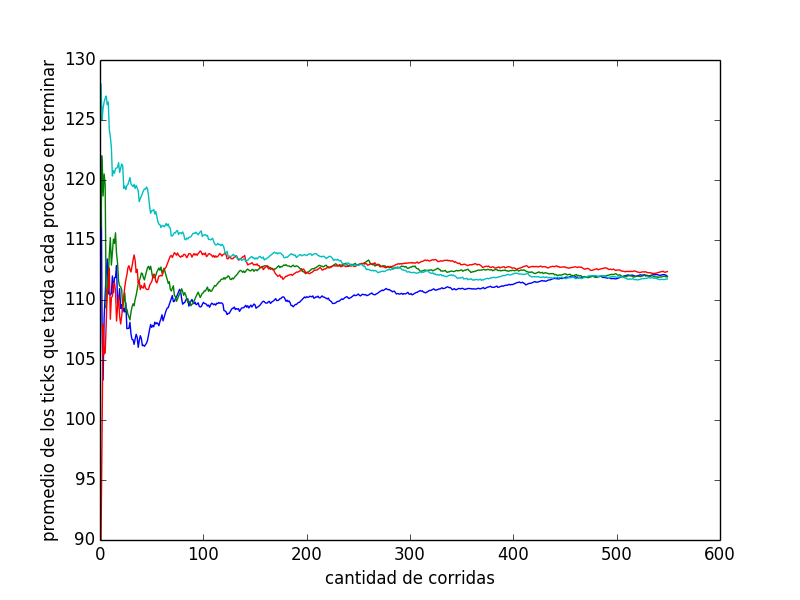
\includegraphics[width=\textwidth]{../experimentacion/ej9-fairness/tiempo_final/prueba-tiempo-final.png}
\caption{Tiempo de ejecución de cuatro procesos idénticos}
\end{figure}


Los tiempos de ejecución arrancan muy dispares. Primero se acercan hacia un valor intermedio de manera exponencial, luego van convergiendo lentamente hacia el mismo valor, en éste caso aproximadamente 112. Se puede concluir de forma fehaciente que a medida que la cantidad de corridas aumenta, la ecuanimidad del LotteryScheduler se acerca a la perfección.








\clearpage
\subsection{Ejercicio 10}

Los $compensation\ tickets$ están diseñados para compensar un proceso que no llegó a completar su quantum al ser bloqueado, por ejemplo. Es un mecanismo sencillo de implementar en un $Lottery Scheduler$ pero que puede ser poco factible en otros schedulers. En la siguiente experimentación se puso a prueba que papel toma este mecanismo en garantizar la ecuanimidad del scheduling.

Se planteó el siguiente escenario:
\begin{itemize}
    \item 5 procesos \texttt{TaskCPU(30)}
    \item 5 procesos \texttt{TaskAlterno(0, 100, 30)} es decir, se bloquean por 100 ticks y luego usan el CPU por 30 ticks
    \item quantum de 10 ticks
    \item todos los procesos lanzados al mismo tiempo
\end{itemize}

El interrogante que se plantea es si los procesos que hacen las llamadas bloqueantes van a terminar su ejecución mucho después que los procesos que solo usan el CPU. Se corrió el experimento sin valerse de los $compensation\ tickets$ y luego haciendo uso de ellos.

\begin{figure}[H]
\centering
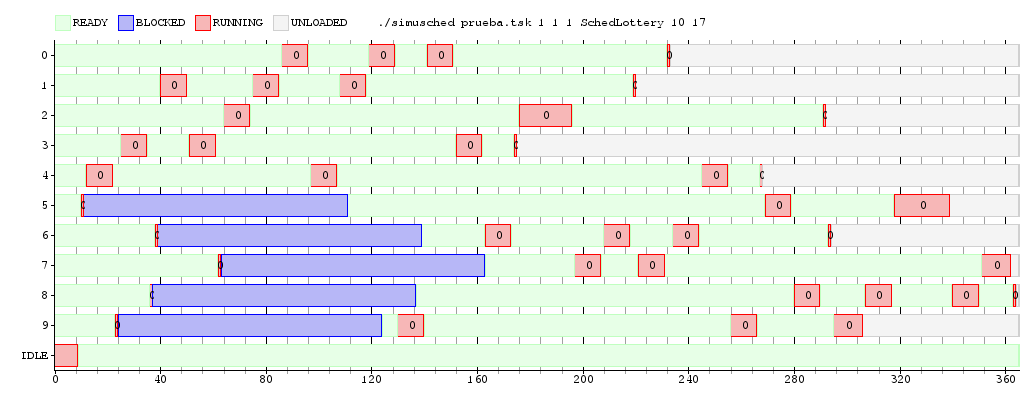
\includegraphics[width=\textwidth]{../experimentacion/ej10-compensation/gant-sin.png}
\caption{Diagrama de Gantt sin $compensation\ tickets$}
\end{figure}

Como es de esperar, mientras los procesos de IO se bloquean, el resto es elegido con frecuencia y puede correr gran parte de sus 30 ticks de CPU. Cuando los procesos de IO se desbloquean, el tiempo de CPU se divide equitativamente entre todos, pero, como los procesos de CPU ya habían corrido bastante tiempo previamente, terminan antes.

\begin{figure}[H]
\centering
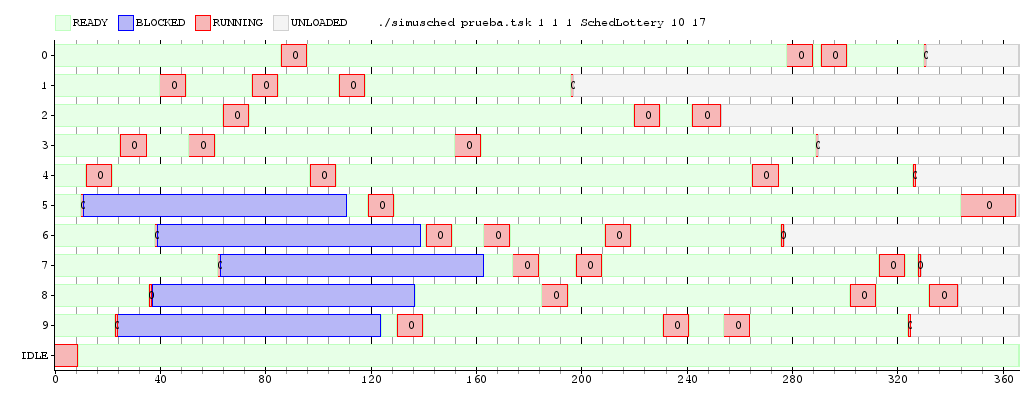
\includegraphics[width=\textwidth]{../experimentacion/ej10-compensation/gant-con.png}
\caption{Diagrama de Gantt con $compensation\ tickets$}
\end{figure}

En este caso la ejecución comienza igual. Sin embargo, al desbloquearse los procesos de IO, se puede percibir otra tendencia. Como para realizar la llamada bloqueante utilizaron solo un tick de procesador, $1/10$ del quantum asignado, se les entregan 10 tickets en vez de 1. En la siguiente ronda de loterías, estos procesos ejecutan casi como si estuvieran solos. Tienen $5/55$ tickets cada uno contra $1/55$ de los procesos de CPU. Al salir seleccionados, vuelven a tener 1 ticket cada uno y el resultado del lottery se empareja. Como consecuencia los procesos terminan más cerca unos de otros.

Este resultado se puede cuantificar en el siguiente gráfico.

\begin{figure}[H]
\centering
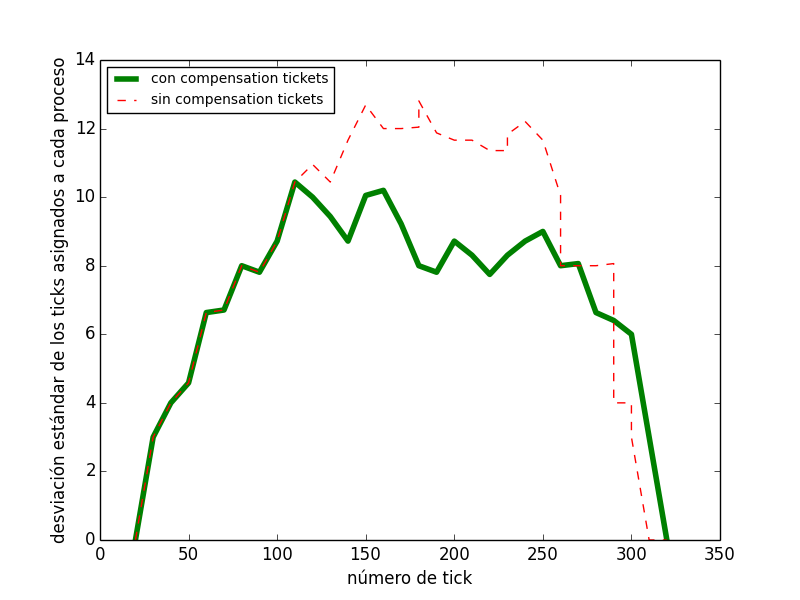
\includegraphics[width=0.7\textwidth]{../experimentacion/ej10-compensation/plot-comparativa.png}
\caption{Comparación de $fairness$ con y sin $compensation\ tickets$}
\end{figure}

La evolución del desvio estándar comienza igual, hasta el tick 120 donde se liberan los procesos bloqueados. A partir de ese momento la corrida con $compensation\ tickets$ presenta una desviación observablemente menor. Lo que se concluye es que los $compensation\ tickets$ son un mecanismo que se puede implementar fácilmente en el $Lottery Scheduler$, que no implican un $overload$ excesivo en el scheduling y que permiten aumentar corroboradamente la ecuanimidad en la asignación de recursos.

\end{document}
